%%%%%%%%%%%%%%%%%%%%%%%%%%%%%%%%%%%%%%%%%%%%%%%%%%%%%%%%%%%%%%%%%%%%%%%%%%%

\documentclass{standalone}

\usepackage{mathptmx}
\usepackage{tikz}
\usetikzlibrary{external}
\tikzexternalize{triangle}

%% We default to Times.
\renewcommand{\rmdefault}{ptm}
\renewcommand{\ttdefault}{pcr}
%% Enable Times/Palatino main text font.
\normalfont\selectfont

%% A right-angled triangle.

\begin{document}

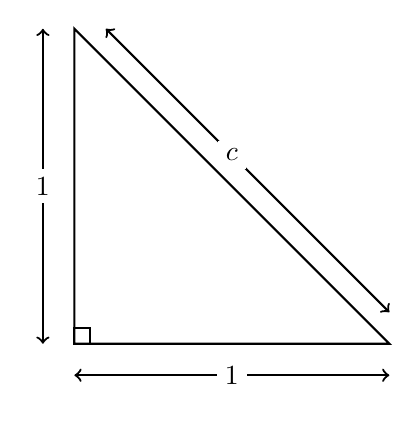
\begin{tikzpicture}[%%
  arrowLabel/.style={inner sep=3pt,fill=white},%%
  arrowStyle/.style={<->,thick,draw},%%
  lineStyle/.style={-,thick},%%
  triangleStyle/.style={-,thick,draw}
]
%%
%%
\pgfmathsetmacro{\dx}{0.2}
\pgfmathsetmacro{\dy}{\dx}
\pgfmathsetmacro{\xA}{0}
\pgfmathsetmacro{\xB}{4}
\pgfmathsetmacro{\yA}{4}
\pgfmathsetmacro{\yB}{0}
\coordinate (A) at (\xA,\yA);
\coordinate (B) at (\xB,\yB);
\coordinate (C) at (\xA,\yB);
%%
%%
%% Draw the right-angled triangle.
\path[triangleStyle] (A) -- (B) -- (C) -- cycle;
\draw[lineStyle] (C) rectangle (\xA+\dx,\yB+\dy);
%% Label the length of the horizontal segment.
\draw[arrowStyle] (\xA,\yB-2*\dy) -- (\xB,\yB-2*\dy);
\node at (\xB/2,\yB-2*\dy) [arrowLabel] {$1$};
%% Label the length of the vertical segment.
\draw[arrowStyle] (\xA-2*\dx,\yB) -- (\xA-2*\dx,\yA);
\node at (\xA-2*\dx,\yA/2) [arrowLabel] {$1$};
%% Label the length of the hypotenuse.
\draw[arrowStyle] (\xA+2*\dx,\yA) -- (\xB,\yB+2*\dy);
\node at (\xB/2,\yA/2+2*\dy) [arrowLabel] {$c$};
\end{tikzpicture}

\end{document}
